\documentclass[a4paper,10pt,fleqn]{article}

%%% Packages
\usepackage{graphicx} % use graphics
\usepackage{color}
\usepackage{amsmath}
\usepackage{amsfonts}
\usepackage{url}
\usepackage{multicol}

% Dansk opsætning (husk renew commands efter begin)
\usepackage[utf8]{inputenc}
\usepackage[danish]{babel}
\usepackage[T1]{fontenc}
\usepackage[lofdepth=1]{subfig}

%\usepackage{algorithm}
%\usepackage{algorithmic}

%%% Modify page layout
\setlength{\textwidth}{160 mm} % line width
\setlength{\oddsidemargin}{0 mm}  % left margin
\setlength{\topmargin}{-1.5 cm} % top margin
\setlength{\textheight}{25.0 cm} % page width
%\pagestyle{empty} % remove page numbers
\setlength{\parindent}{0 mm} % indent at the beginning of a paragraph
\setlength{\parskip}{2 mm} % vertical distance between paragraphs

% Text fonts
\usepackage{palatino}

\usepackage[hyperindex=true,pdftitle={},pdfauthor={},colorlinks=true,
pagebackref=false,citecolor=blue,linkcolor=blue, urlcolor=blue, plainpages=false,
%pagebackref=false,citecolor=black,linkcolor=black, urlcolor=black, plainpages=false,
pdfpagelabels]{hyperref} % colourlinks=false for printing

\usepackage[round,colon,authoryear]{natbib}

\begin{document}

\Large
\textbf{Unmanned Aerial Systems Techology (RMUAST) Spring 2017 \\ University of Southern Denmark}

\Large
\textbf{Team 2}
\normalsize
\\
Programming exercises can be found at \textit{\href{https://github.com/TobiasLundby/UAST}{link}.}

\vspace{3mm}

\LARGE Module 1: Global Navigation Satellite Systems 


\normalsize
%\vspace{10mm}

\section{Exercises}

\subsection{Global Navigation Satellite Systems}
Besides GPS there are a number of other GNSS.

\subsubsection{GLONASS}
Equivalent to GPS but made by Russia and has been in development for approximately as long as GPS. There are a lot of GLONASS satellites  but they tend to fail more often compared to GPS and it is therefore rarely used exclusively.

\subsubsection{Galileo}
Similar to GPS but made by the EU and is compatible with GPS. Became operational in December of 2016 but first reaches full operation in 2019.

\subsubsection{Compass}
China's answer to GPS but only sparse information has been released and only 1 satellite has been launched.

\subsubsection{QZSS}
Japan's answer to improving GPS within the Japanese islands and consists of 3 geosynchronous satellites. These satellites have a special orbit so they seem to allways be over Japan.

Source: GNSS\_for\_Vehicle\_Control\_2010.pdf

\subsection{GPS architecture}
\subsubsection{Space Segment}
\textit{The Space Segment} consist of at least 4 satellites that are responsible for transmitting information made available by \textit{the Control Segment} as radio signals and storing the information to facilitate retransmission. 

\subsubsection{Control Segment}
\textit{The Control Segment} is responsible for processing measurements such as calculating clock errors and estimating satellite orbits such that the navigation message (including correction information) for each satellite can be generated. It consists of a Master control station, Ground Antennas, and Monitor Stations. The master control station is responsible for the processing and the information is afterwards uploaded via Ground Antennas.

\subsubsection{User Segment}
\textit{The User Segment} are GPS receivers which are responsible for receiving GPS signals, calculating calculating pseudoranges (distance to satellites), and finally solving equations to determine their respective position coordinates.

Source: \url{http://www.navipedia.net/index.php/GPS_Architecture}


\subsection{GNSS error sources}

\subsubsection{System clock}

A high frequency of the system clock on the receiver is important to get a high precision on the position mesurment.

The errors is obtained from inaccuracy in the system clock of the gps receiver and in differences in weather condition.

\subsection{Dilution of Precision (DOP)}
What are GDOP, PDOP, HDOP and VDOP?

"GDOP describes the accuracy degradation of the position solution due solely to the relative positions of the satellites."~\textit{from source}

GDOP includes components describing the degradation in different dimensions; namely position, horizontal and vertical.

PDOP: positional DOP (3 dimensions)

HDOP: horizontal DOP

VDOP: vertical DOP

There is also TDOP, which is time DOP.


Source: GNSS\_for\_Vehicle\_Control\_2010.pdf

Illustration of DOP, see \url{https://en.wikipedia.org/wiki/Dilution_of_precision_(navigation)}

\subsection{GNSS accuracy}

\subsubsection{SPS}
For 3D positioning using SPS a minimum of four satellites is used. The satellites emits its time and position. The GPS receiver calculates the 3D position based on the distances from the four satalites based on triangulation or multilateration.

The precision of 3.5 meter. see:  \url{https://en.wikipedia.org/wiki/Global_Positioning_System}

\subsubsection{DGPS}
The DGPS system works as SPS but obtain the live distance offset from each satalite using a fixed ground station which knows its position.

This increase the precession down to 2 meter.

\subsubsection{RTK float}
RTK estimates the number of carrier signal periods between the GPS receiver and the satellite. The float version estimates the number of waves using statistical techniques to get a best estimate and uses that for positioning. The accuracy is approximately 40 cm and 20 at its best since the ambiguity problem is not solved. 4 satellites are required.

Source: http://www.oxts.com/what-is-inertial-navigation-guide/what-is-rtk/

\subsubsection{RTK fixed\/integer}
RTK fixed mode differs from float by trying to solve the integer ambiguity problem. The output from this approach is not used until the problem is solved. The precision is 1 mm and requires 5 satellites. 

Source: http://www.oxts.com/what-is-inertial-navigation-guide/what-is-rtk/

The PRN pulse width is 300 meters long and the carrier frequency is about 19 cm long.

The distance error is about 0.5 meters for PRN and 1mm fir the phase.

\subsection{RTK-GNSS}
The integer ambiguity is the number of whole cycles/periods of the carrier frequency. Additionally there is a fraction of a cycle (of the carrier frequency) but this is the relative carrier phase. The ambiguity exists because it is not an integer amount but actually an integer plus the fraction from the relative carrier frequency.

\section{Programming Exercises}

\subsection{Universal Transversal Mercator (UTM) accuracy}
Converting a geodetic coordinate (lat 55.36732 and lon 10.43192) to UTM results in 32 U 590755.78902e 6136600.87185n. Adding 1km to either the eastern or northern coordinate results in the following error:

\begin{enumerate}
\item 1.5919519233 m when adding to the eastern direction
\item 3.7590204766 m when adding to the northern direction
\end{enumerate}

The size of the resulting error, in the corresponding direction (when only adding 1km to one of the directions), depends on the position on the earth.

\subsection{National Marine Electronics Association (NMEA) 0183 data}
The script \textit{exercise4\_3.py} parses the \textit{nmea\_trimble\_gnss\_eduquad\_flight.txt} to plot altitude and number of tracked satellites with respect to time. The results are given in figures~\ref{fig:altitude_plot} and \ref{fig:satellite_plot}. The script also creates a KML-file for plotting the drone track and static accuracy data for \textit{nmea\_ublox\_neo\_24h\_static.txt} respectively in figures~\ref{fig:drone_track} and \ref{fig:satellite}.

\begin{figure}[]
    \centering 
    \subfloat[][Altitude vs. time]{
        \label{fig:altitude_plot}
        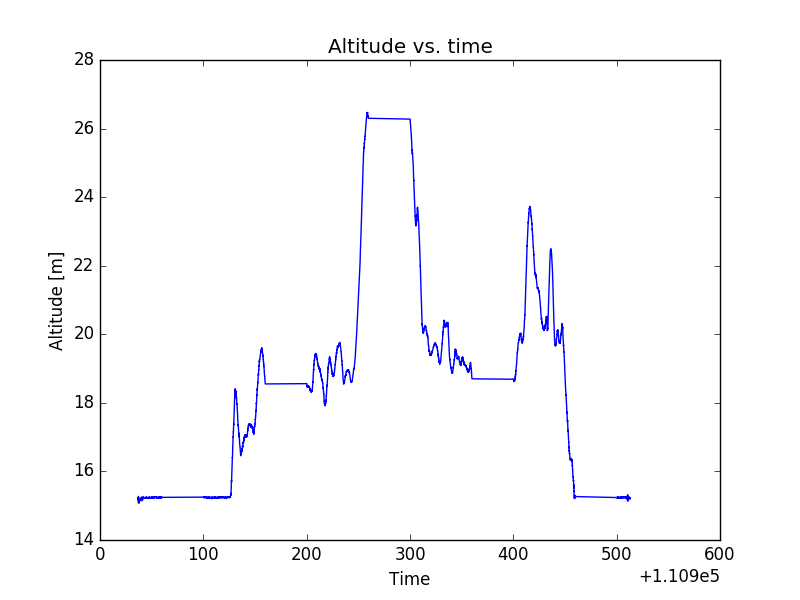
\includegraphics[width=0.45\textwidth]{./graphics/altitude_vs_time.png}}
    \qquad
    \subfloat[][Tracked satellites vs. time]{
        \label{fig:satellite_plot}
        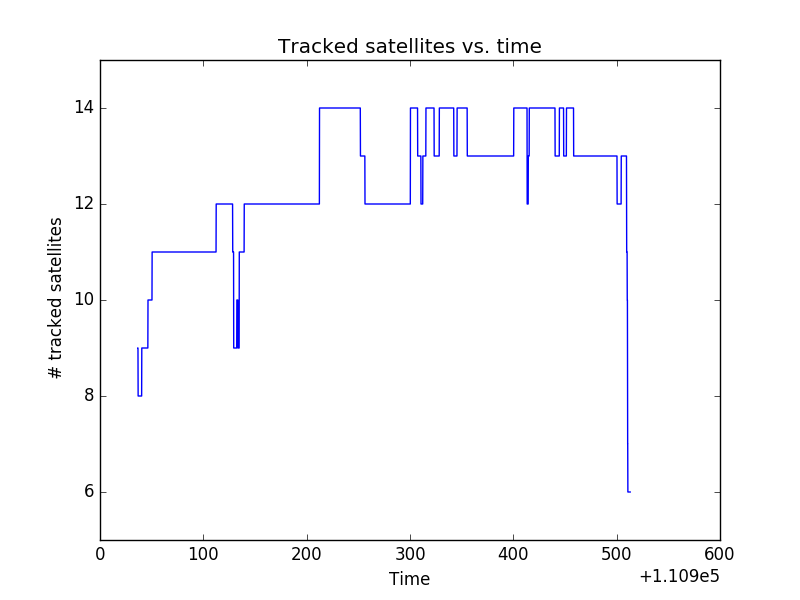
\includegraphics[width=0.45\textwidth]{./graphics/tracked_satellites_vs_time.png}}
    \caption[]{Results from parsing \textit{nmea\_trimble\_gnss\_eduquad\_flight.txt}.} 
    \label{fig:id_overall}
\end{figure}

\begin{figure}[]
    \centering 
    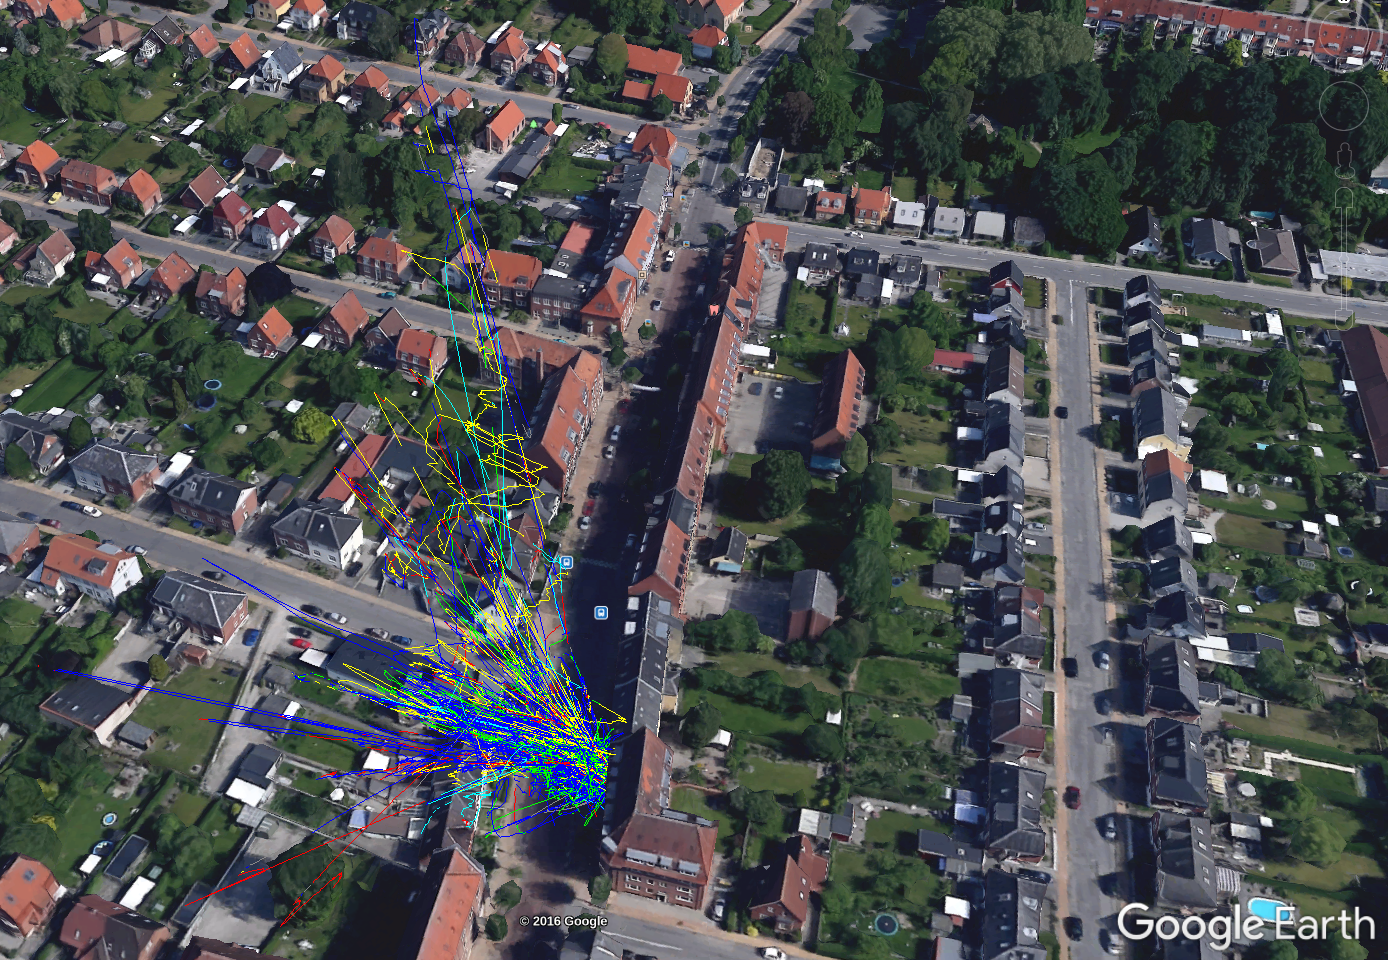
\includegraphics[width=0.7\textwidth]{./graphics/drone_track.png}
    \caption[]{Plot of drone track from \textit{nmea\_trimble\_gnss\_eduquad\_flight.txt} in Google Earth.} 
    \label{fig:drone_track}
\end{figure}

\begin{figure}[]
    \centering 
    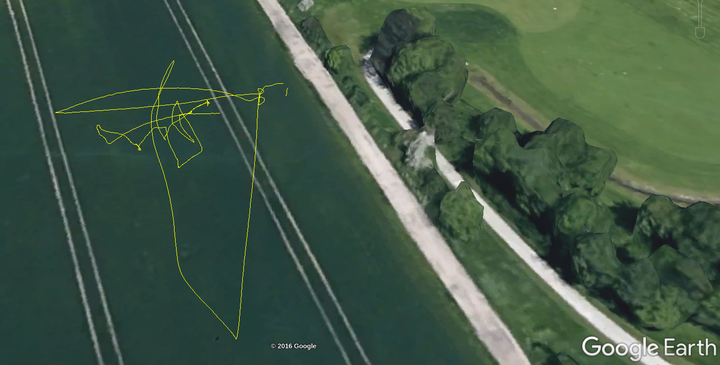
\includegraphics[width=0.7\textwidth]{./graphics/GNSS_accuracy.png}
    \caption[]{Plot of static GNSS accuracy in Google Earth. Color coding with reference to PDOP: Green (less than 2), blue (less than 3), yellow (less than 4), cyan (less than 5), grey (less than 6), and red (above 6).}
    \label{fig:satellite}
\end{figure}

\newpage
\section{Responsibility}
\begin{table}[h!]
\centering
\begin{tabular}{l|l|l|l|}
\cline{2-4}
 & \multicolumn{1}{c|}{\textbf{Mathias}} & \multicolumn{1}{c|}{\textbf{Rasmus}} & \multicolumn{1}{c|}{\textbf{Tobias}} \\ \hline
\multicolumn{1}{|l|}{\textbf{Lab1}} & 33\% & 33\% & 33\% \\ \hline
\end{tabular}
%\caption{My caption}
\label{my-label}
\end{table}

\end{document}
